
%         %!TEX root = ../Thesis.tex
\chapter{Introduction}\label{cha:introduction}
%
% This introductory chapter will briefly provide context for the material/results presented in this report and give motivation and a description of the problem to be solved. A literature review summarizes existing relevant knowledge and establishes the foundation of the later control system. A list of assumptions then defines the scope of the work. Finally, the contributions of the thesis are defined and elaborated.

This is a master thesis written in cooperation between NTNU and Hymatek Controls. Hymatek Controls is located in Oslo and delivers equipment and control systems to hydroelectric power plants worldwide. Hymatek is increasing its focus on condition monitoring and anomaly detection and has acquired a large dataset containing data from a five year period for $27$ hydroelectric power plants. The goal of this thesis is to find possible use cases for condition monitoring in the provided dataset, research possible techniques and implement some of them in the found use case. Since this is a new research area for Hymatek, this thesis will cover a wide range of aspects. 

This chapter provides an introduction to the work that has been done, describing the motivation and problem description for the thesis. A literature review looks into state of the art techniques used for condition monitoring. Finally, the outline of the report is presented. 


\section{Motivation}\label{sec:motivation}

% % What is the motivation for considering the problems/question that you approach in your work? Why is this an interesting problem? The motivation should instead describe why it is interesting from a societal point of view, and/or from a scientific point of view.

There is an increasing need for stable renewable energy in Norway, Europe and worldwide. According to \cite{Statkraft2009} $99\%$ of the Norwegian power production comes from hydroelectric power plants. Norway has almost $50\%$ of Europe's hydroelectric capacity. According to \cite{Statkraft2009} hydroelectric power is one of the most stable and cleanest energy sources one can find. Hydroelectric power plants have a high investment cost, but according to \cite{Selak2014} operation and maintenance costs are as low as 2\% of the cost of the initial investment, this makes it one of the cheapest energy sources available. As many European countries are transitioning into renewable energy sources, the need for stable and controllable power sources grows. Both wind and solar power production are dependent on weather conditions, and their production capacity can change quickly and unexpectedly. Norway has been called Europe's renewable battery due to its hydroelectric capacity, and the power export capacity is growing. By 2021 Norway and Great Britain will be connected through a new underwater power cable. This shows how Norway is becoming a part of a more complex energy market. As the export capacity grows, green energy from Norway can be supplied to reduce the consumption of fossil energy from for example coal from the European continent. This means that increased productivity and efficiency in hydroelectric power plants effectively can help make the green shift in the European power production happen. 

One way to increase a plant's productivity is to ensure that it is operable at all times. However, this is not possible since one has to perform maintenance on all parts of a plant. Planned maintenance is however not the only reason for a power plant stopping down. Components can break down outside of their service interval, leading to unplanned downtime. This is of course not only a case for hydroelectric power plants but more or less any industry or factory. Unplanned downtime is expensive for the energy company that operates the plant, and depending on the time of year and the duration of the breakdown, the cost can have a significant impact on their operation. Finding a way to avoid these breakdowns, and replacing unplanned maintenance with planned maintenance, is something all energy companies find interesting. A hydroelectric power plant contains several large components such as turbines, generators, transformers, hydraulic systems, valves, pipes, and so on.  As an addition comes all the equipment needed to operate the plant. Keeping spare parts for all components would require enormous storage capacity, and ties considerable assets due to the cost of the spare components. Many components do not need to be often replaced, hence the spare can be left unused in storage for many years, and may even never be replaced. This is not an optimal solution. 

Another approach is to try to eradicate unexpected breakdowns. This means that one needs to detect that a component is decaying so that one can plan an overhaul or replacement before it breaks down. Depending on the situation and the component, if a component breaks down, there is a risk that it can take several others with it. If a bearing on a turbine shaft breaks down, there is a risks that the damage will spread to the bearing on the other side of the shaft, and even to the turbine and generator. Continuous analysis of the condition of the bearing could help avoid this issue. This is known as condition monitoring. In its most complete form, condition monitoring gives an insight into the condition of the monitored components, giving an estimate to the remaining lifetime of the component. Introducing condition monitoring could help reduce the number of breakdowns, as components can be replaced before breaking.

There are many good reasons for pursuing the topic of this thesis, on a personal level it is motivating to work with real-world data, to learn the difference between theoretical and practical engineering. Looking for solutions that will improve the operation of a hydroelectric power plant, which can give even more clean energy is also motivating. Additionally, the fact that possible solutions found for the specific cases analyzed most likely can be adapted to other industries is also very motivating. 

% An attempt of classifying the wear of the guide vanes on a Francis turbine was performed in my project thesis.  


% This triggered my interest in the possibilities of information found in data. 
% Looking into different possible techniques for condition monitoring that can be utilized on a real-world dataset will give
% As the world becomes more and more digitized, one can either keep up or be left behind. Condition monitoring is seen as an important part of the future portfolio of Hymatek Controls and a necessary addition to continuing their growth into the future. 

% \section{Contributions}
    


\section{Problem definition}

% Korleis oppsto problemstillinga? dreiv å såg gjennom feiloggen etter interesssante feil. Såg då at det var problemer med nålstryinga for hjartdøla. Starta så å undersøke dataen, og fant etterkvart ut at det er 2 anlegg til som har nålstyring. Dei hadde derimot ikkje raportet feil med nålene, noko som gav meg grunn til å tenke at dei har normal oppførsel. Då kunne eg og starte å samanlikne data mellom kraftverka for å sjå kva som er unormal og normal oppførsel.

Hymatek provided no exact problem definition, they provided a dataset containing process-data from $27$ hydroelectric power plants for the period $2013-2017$, and gave no restriction on which plants and cases to investigate. A historical incident log was also provided for all plants, with varying level of detail. Based on this, the problem definition was split into three main parts. As this is a thesis built upon an unknown dataset with unknown quality, an important factor is to recognize what the data can be utilized for, and what improvements that could/ need to be done to make the data analysis more extensive. Ideally, the result of the thesis will be a system for condition monitoring and anomaly detection for a real-world case found in the dataset. However, since Hymatek is still in the start-up phase of its condition monitoring research, all experiences from this thesis are valuable. The goal is that thesis can be used as a basis for further condition monitoring case analysis. The three parts are as follows: 

\begin{itemize}
    \item Finding methods for anomaly detection. Finding methods for feature extraction and dimensionality reduction to be used in addition to the anomaly detection techniques.
    \item Data preparation and case extraction. The provided data is not ready for analysis, and one needs to extract datasets for each of the plants. Once the data is in a format that can be analyzed, the historical data from the plants and the datasets need to be analyzed to build a case for testing of the anomaly detection techniques. 
    \item Analyzing the case using the techniques found. Emphasize on how the different techniques perform, and what can/needs to be done to improve the performance. 
\end{itemize}


% \section{Literature review}\label{sec:review}
    

% Start writing about the articles I have already read, can always delete it if it is not relevant in the end. 
%     \subsection{Timeseries forecasting}\label{sec:time_series_forecasting}
    
%     \subsection{One class support vector machine novelty/anomaly detection}\label{sec:ocsvm_novelty_detection}
    
%     \subsection{Neural network novelty/anomaly detection}\label{sec:nn_novelty_detection}
    
%     \subsection{The data set}\label{sec:the_data}
%     The data is provided by Hymatek controls and is collected from more than 30 hydroelectric power plants around Norway, in the period between $01.01.2014$ and $01.07.2017$. 

\section{Limitations}\label{sec:assumptions}
    Since the thesis span over many different research areas, only one case will be analyzed, even if it should be possible to find several more from such an extensive dataset. Also, only a subset of the suggested techniques will be chosen for analysis, spanning from easy to more complex. There might be algorithms not tested that could be useful for the given case. The techniques are chosen in cooperation with Hymatek. 
    
    Availability of computing power and memory also introduces constraints to the analysis. All analysis is performed on a desktop from dell provided by NTNU. This means that no analysis will be performed using the full datasets, they will be reduced by either feature selection or dimensionality reduction. 
    
    Condition monitoring is a broad field, and creating a full-scale condition monitoring system is too comprehensive. The thesis will, therefore, focus on anomaly/novelty detection for the given case. This means that one will train different techniques on normal operation data, and verify how well the different techniques can detect the anomaly found for the specific case. 
    
\section{Hydroelectric power production}\label{ref:sec_hydropower}
    $99\%$ of the Norwegian power production comes from hydroelectric power plants. Hydroelectric power is clean, reliable and once built, it produces cheap energy. According to \cite{Statkraft2009} no other types of power plants have longer expected lifetime and higher efficiency than hydroelectric power plants. Statkraft also states that countries with the highest increase in energy demand are also countries with the highest unused potential for hydroelectric power. This means that hydroelectric power production can play a significant role in the hunt for meeting the global energy demand. There are many old power plants today, so there are also possibilities for modernization and extensions of already existing plants. 
    
    The principal behind hydroelectric power is simple. It utilizes the energy in running water, converting it to electric energy through a turbine. According to \cite{Paish2002}, there are two main types of turbines, impulse and reaction. The difference between the two types is how they create the rotational force. The impulse turbine rotor runs in air, and the rotational force is created by a water jet lead onto the turbine blades. The reaction turbine is submerged in water, and the rotational force comes from a lift force created by the oncoming water flow. For the impulse turbine, kinetic energy generates the rotational force, for the reaction both kinetic and pressure energy generates it. When the water hits the turbine blades, the water pressure is reduced to atmospheric pressure, and all pressure energy is converted to kinetic energy. For the reaction turbine, which is submerged in water, the water pressure is still high, meaning that one needs a casing which is sealed from atmospheric pressure. 
    
    % \begin{figure}
    %     \centering
    %     \includegraphics{}
    %     \caption{Principal behind reaction and impulse turbines}
    %     \label{fig:my_label}
    % \end{figure}
    
    
    The two most common turbine types are Francis and Pelton. The type used is defined by the size of the flow and the head of the water. Whether the turbine will be producing power only at optimal flow, or if it will be used for power production over a broader range is also a criterion. 
    
    
    
    \subsection{Pelton turbines}\label{subsec:pelton}
        
        The Pelton turbine is the most common impulse turbine. Water is lead onto to the turbine through a series of needles or valves. The turbine has a set of buckets located on the turbine wheel which splits the water jet in two, where each half is deflected back and falls into a discharge channel, \cite{Paish2002}. A cross-section of a Pelton turbine is seen in Figure \ref{fig:pelton_turbine}. As one can see the needles are divided equally around the turbine. The amount of produced power is controlled by the number of active needles, and by regulating their opening. Figure \ref{fig:pelton_bucket} shows how the buckets are designed. Where the water jets hit the buckets is easily verifiable by looking at the corroded parts of the buckets. The needles are controlled by a hydraulic system, which is controlled by the power plant control system. To ensure an even momentum on the turbine, all active needles should have the same opening. 
        
        
        \begin{figure}
            \begin{minipage}[b]{0.49\linewidth}
                \centering
                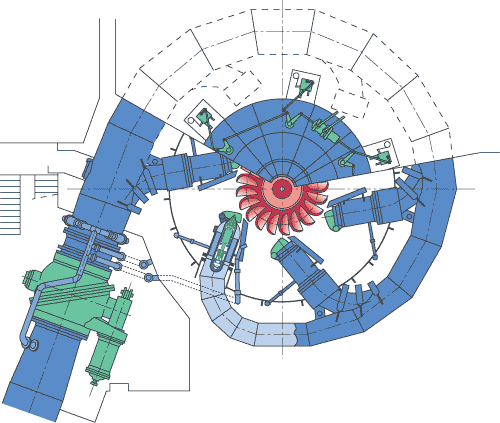
\includegraphics[width = 0.9\textwidth]{report/figures/introduction/pelton.png}
                \caption{Cross section of a Pelton turbine with $6$ needles. By Voith Siemens Hydro Power Generation.\footnote{Licensed under GFDL, Wikimedia Commons \url{https://commons.wikimedia.org/wiki/File:S_vs_pelton_schnitt_1_zoom.png}}} 
                \label{fig:pelton_turbine}
            \end{minipage}
            \hfill\vline\hfill
            \begin{minipage}[b]{0.49\linewidth}
                \centering
                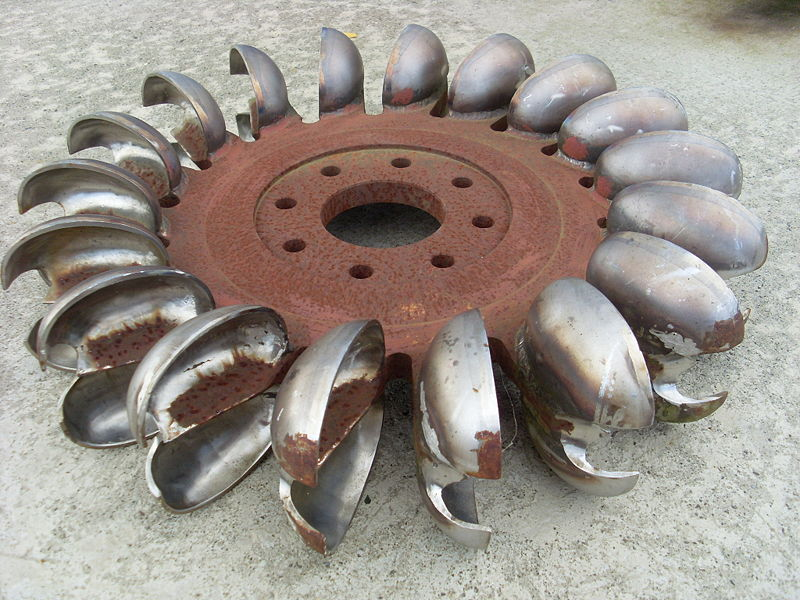
\includegraphics[width = 0.9\textwidth]{report/figures/introduction/pelton_bucket.jpg}
                \caption{A Pelton turbine wheel, the split buckets are easily visible. By Zedh. \footnotetext{Licensed under CC-BY-SA, Wikimedia Commons. \url{https://commons.wikimedia.org/wiki/File:Pelton_400kW_roue_1.JPG}}} 
                \label{fig:pelton_bucket}
            \end{minipage}
        \end{figure}
        
        
    
    \subsection{Francis turbines}\label{subsec:francis}
        The Francis turbine is a reaction turbine. The water is lead onto the turbine through a set of guide vanes connected to the spiral casing, and lead out from the center of the turbine. Guide vanes control the amount of water lead to the turbine, and hence the amount of produced energy. A cross-section of a Francis turbine is seen in Figure \ref{fig:francis}. All guide vanes have the same opening and are controlled through a ring mounted on the top of the turbine. Figure \ref{fig:guide_vanes} shows a hydraulic actuator used to control the ring that operates the guide vanes. As for the Pelton turbine, the hydraulics is again controlled by the plant's control system. \cite{Aasnes2017} tries to classify the condition of the guide vanes in a Francis turbine using different machine learning methods such as support vector machines (SVM), neural networks (NN) and regression.   
        
        \begin{figure}
            \begin{minipage}[b]{0.49\linewidth}
                \centering
                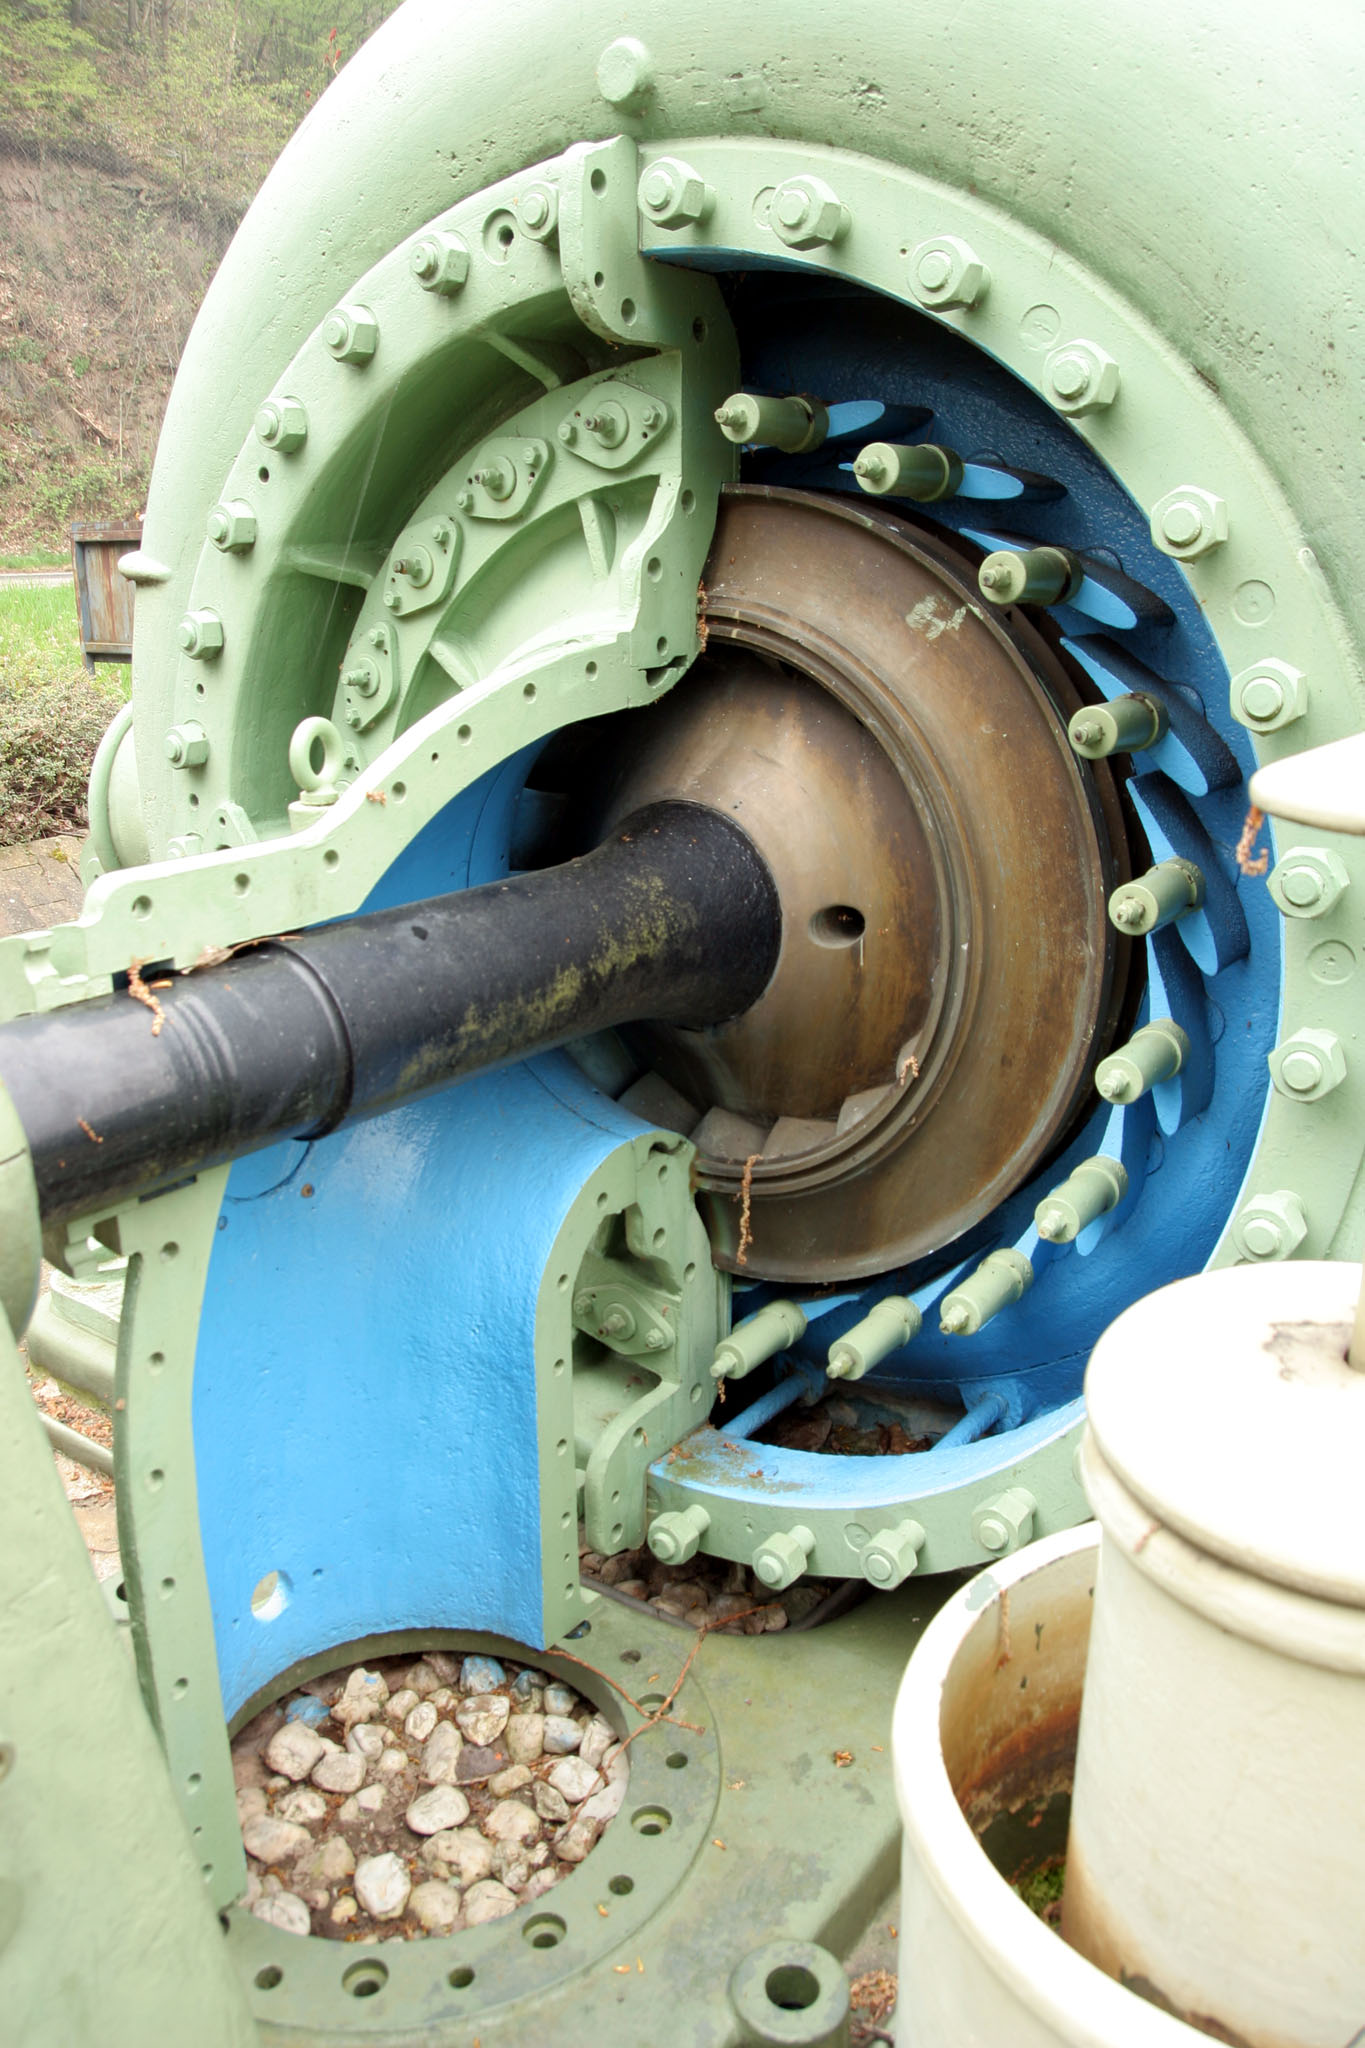
\includegraphics[width = 0.9\textwidth]{report/figures/introduction/francis_turbine.jpg}
                \caption{Cross section of a Francis turbine. The guide vanes are seen in almost closed position. By Armin Kübelbeck.\footnote{Licensed under CC-BY-SA, Wikimedia Commons, \url{https://commons.wikimedia.org/wiki/File:Fankel_Francisturbine_01.jpg}}}
                \label{fig:francis}
            \end{minipage}
            \hfill\vline\hfill
            \begin{minipage}[b]{0.49\linewidth}
                \centering
                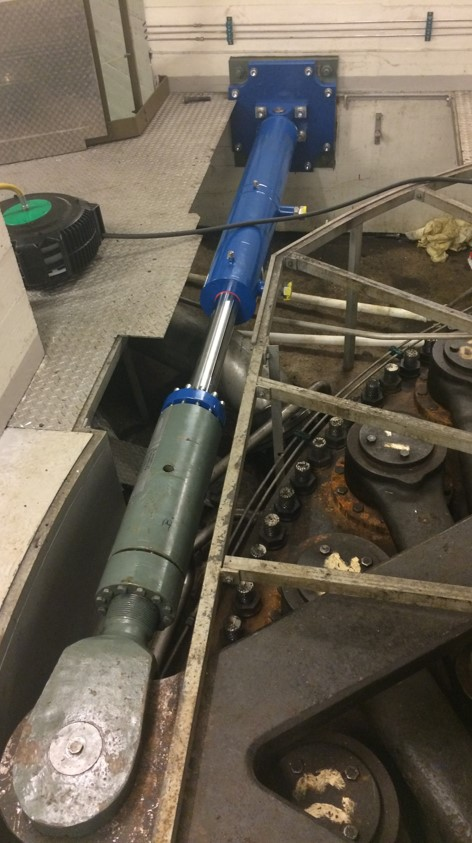
\includegraphics[width = 0.9\textwidth]{report/figures/introduction/servo1(1).jpg}
                \caption{Hydraulic actuator for guide vane control. The actuator is mounted to a ring that controls the guide vane opening. Courtesy of Hymatek Controls}
                \label{fig:guide_vanes}
            \end{minipage}
        \end{figure}
        
    \subsection{Other plant equipment}
        There are several other large components in a hydro-electrical power plant. Among them are;
        \begin{itemize}
            \item Generators
            \item Transformers
            \item Coolers
            \item Hydraulic systems
        \end{itemize}
    
    \section{Condition monitoring for hydroelectric power plants}\label{sec:cm}
        \cite{Selak2014} presents a complete condition monitoring and fault detection system for hydroelectric power plants, covering everything from data acquisition to fault detection methods. Cost reduction, increase in equipment availability and increased performance are presented as the benefits of introducing condition monitoring. They propose using condition monitoring in addition to preventive maintenance and claim that it is the most comprehensive maintenance scheme available. Data is transferred to a virtual diagnostics center, where a support vector machine (SVM) is used to diagnose the data. The proposed condition monitoring system is separated into six steps; data acquisition, data analysis and storage, data transferring, data selection, SVM training and SVM testing. It is proposed to sample data in four different ways to reduce the amount of data stored; periodically at a predefined sampling rate, when signal values exceed a threshold, during transients and sudden events. 
        
        Data that represents all known failure modes and normal data is needed to train a SVM to for fault diagnostics. The work is restricted only to include two variables at a time, as this enables scatterplotting variables against each other for visual confirmation of the normal operation. The training cases separate data into four different datasets; All input data, removing low power operations, removing high water flow operations and removing transients between operation regimes. Experts extracted 44 causalities that can be traced to a pair of process variables. Abnormal data is created as a complement to the normal data, by fitting an oversized boundary to the data from normal operation. As the SVM detector is only trained on two classes, data is only evaluated as normal or abnormal. It is claimed that two-dimensional models are sufficient to catch all known failure modes. The choice of using SVM is supported by \cite{Widodo2007} that presents that SVM has been successfully used in the industry for several different use-cases. 
        
        \cite{Molina2000} introduces two neural network (NN) approaches to integrate into a decision system for hydroelectric power plant management. An expert system, an NN for acoustic prediction and an NN for predictive maintenance are proposed integrated into one system. It is argued that there are non-linear plant dependencies undetectable for a human expert, that the NN can find. As the expert system tries to mimic the response of a human operator, the system suffers from the same limitations as a human operator. Interpreting an expert system is however much more straightforward than interpreting an NN. Therefore a hybrid system is proposed, benefiting from the best of both worlds. The expert system and the NN for predictive maintenance depend on process data from the plant. The NN for acoustic prediction is fed with data recorded from sensors not used in the two other cases. 106 process variables are available for analysis, all are given as input to the NN, but to mimic the limitations of a human operator, the expert system is only considering 15 variables at a time. The NN for predictive maintenance needs data that represent both normal and abnormal data, for all known failure modes. A particular procedure combining expert knowledge and NNs are used to create data vectors with values for all 106 variables for the given errors created by the expert system. The error vectors are used to train the NN. Classes for the acoustic prediction network are created based on an experts classification of the normal and abnormal regime based on the plants generated power. 
        
        The proposed method was applied and test on a plant in Zamora, Spain. It was found that the combination of the NNs and the expert system outperformed a human operator, but the human operator outperformed the methods individually. The NN for predictive maintenance gave the best individual results. The NN for acoustic predictions suffered from variability in the acoustic signals, but showed that it served as a good addition to the two other methods. 
        
        
    
    
    
    \section{Report outline}
    Chapter \ref{cha:litterature} introduces different anomaly detection techniques, and methods for feature selection and dimensionallity reduction. Chapter \ref{cha:implementation} introduces the software and the libraries used in this thesis. Chapter \ref{cha:data} introduces the dataset and the cases analyzed. Chapter \ref{cha:analysis} walks the reader through the analysis before the discussion and conclusion are found in chapters  \ref{cha:discussion} and \ref{cha:conclusions}.  
